\section{Auswertung}
\label{sec:Auswertung}
Jegliche Fehlerrechnung wurde mit der python-Bibliothek uncertainties \cite{uncertainties} absolviert.
Trotz dessen sind die Formeln für die Unsicherheiten in den jeweiligen Abschnitten angegeben.
Allgemeine Rechnungen wurden mit der python-Bibliothek numpy \cite{numpy} automatisiert. 
Die graphischen Unterstützungen wurden mit Hilfe der python-Bibliothek matplotlib \cite{matplotlib} erstellt.\\
\subsection{Verwendete Bauteile} \label{subsec:bauteile}
Die Bauteile der verwendeten Schaltung haben folgende Werte:
\begin{align*}
    L   & = \SI{16.78(9)} {\milli\henry}\\
    C   & = \SI{2.066(6)} {\nano\farad} \\
    R   & = \SI{67.2(2)}  {\ohm}
\end{align*}
\subsection{Bestimmung des Dämpfungswiderstands bei der gedämpften Schwingung}
In der Tabelle \ref{tab:voltage} ist die Spannung mit den dazugehörigen Zeiten aufgetragen.
\begin{table}
    \centering
    \caption{Gemessene Spannungsamplituden in Abhängigkeit von der Zeit}
    \label{tab:voltage}
    \begin{tabular} {S[table-format=4.1] S[table-format=2.2]}
        \toprule
        {$t \mathbin{/} \si{\micro\second}$} & {$U \mathbin{/} \si{\volt}$}  \\
    \midrule
    20      &   16.5\\
    60      &   14.0\\
    97      &   12.5\\
    135     &   10.5\\
    175     &   9\\
    212.5   &   8\\
    252.5   &   6.5\\
    290     &   5.75\\
    330     &   5.\\
    367.5   &   4.\\
    405     &   3.5\\
    442.5   &   3\\
    480.0   &   2.8\\
    520     &   2.4\\
    557.5   &   2\\
    595     &   1.8\\
    632.5   &   1.6\\
    670     &   1.4\\
    707.5   &   1.2\\
    745     &   1\\
    785     &   0.85\\
    822.5   &   0.75\\
    860     &   0.65\\
    897.5   &   0.55\\
    935     &   0.5\\
    972.5   &   0.4\\
    1010    &   0.35\\
    1047.5  &   0.3\\
    1085    &   0.26\\
    1125    &   0.24\\
    1162.5  &   0.2\\
    1200    &   0.16\\
    1237.5  &   0.14\\
    1275    &   0.12\\
    1312.5  &   0.08\\
    \bottomrule
\end{tabular}
\end{table}
\begin{figure}
    \centering
    \caption{Gemessene Spannungsamplituden mit Regression}
    \label{fig:voltage}
    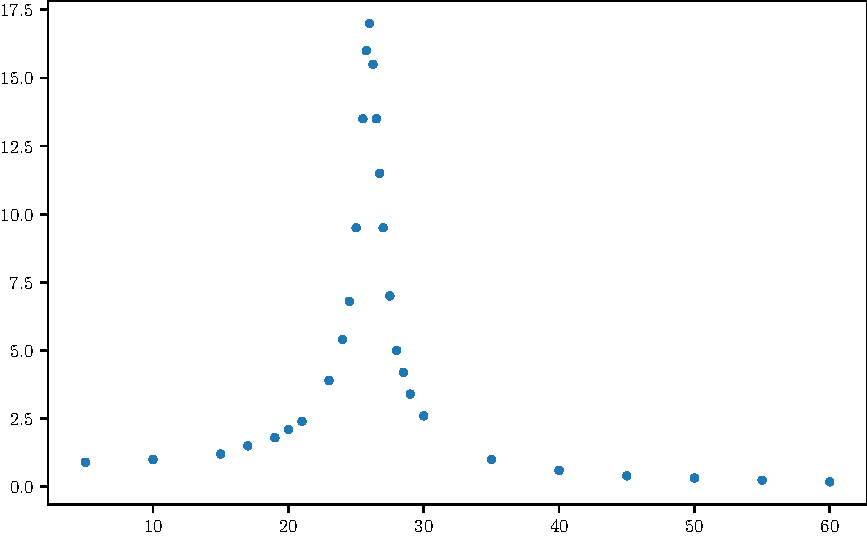
\includegraphics{build/voltage.pdf}
\end{figure}
Um den Dämpfungswiderstand zu bestimmen, ist es von Nöten eine Ausgleichsrechung mit dem $\symup{e}$-Term der Funktion
\eqref{eqn:schwing} durchzuführen.
Die Parameter der Regressionsfunktion
\begin{equation}
    U = U_0 \symup{e}^{-2\pi\mu t}
\end{equation}
lassen sich zu
\begin{align*}
    U_0 &= \SI{17.87(8)}{\volt}\\
    \mu &= \SI{622.51(92)}{\per\second}
\end{align*}
bestimmen.
Mit der Beziehung 
\begin{equation}
    R_\text{eff} = 4\pi\mu L 
\end{equation}
lässt sich der Dämpfungswiderstand $R_\text{eff}$ zu
\begin{equation*}
    R_\text{eff} = \SI{131.26(109)}{\ohm}
\end{equation*}
bestimmen.
Aus dem eben berechneten Dämpfungswiderstand und der Gleichung \eqref{eqn:abklingzeit} kann die Abklindauer zu 
\begin{equation*}
    T_\text{ex} = \SI{255.67(161)}{\micro\second}
\end{equation*}
errechnen.
Der Fehler für den Dämpfungswiderstand ergibt sich mittels Gaußscher Fehlerfortpflanzung zu 
\begin{equation}
    \symup{\Delta} R_\text{eff} = 4\pi \sqrt{L^2 \left( \symup{\Delta} \mu \right)^2  + \mu^2 \left( \symup{\Delta} L \right)^2} \; \text{}.
\end{equation}
Ebenfalls mittels Gaußscher Fehlerfortpflanzung ergibt sich der Fehler der Abklingzeit als
\begin{equation}
    \symup{\Delta} T_\text{ex} = \frac{2}{R_\text{eff}} \sqrt{\left( \symup{\Delta} L \right)^2 + \frac{L}{R_\text{eff}^2} \left( \symup{\Delta} R_\text{eff}  \right)^2 } \; \text{.}
\end{equation}
\subsection{Bestimmung des Dämpfungswiderstandes bei dem aperiodischen Grenzfall}
Mit Hilfe deer Messung wurde ein Dämpfungswiderstand, bei dem der aperiodische Grenzfall eintritt, von
\begin{equation*}
    R_\text{ap} = \SI{4.4}{\kilo\ohm}
\end{equation*}
ermittelt.
\subsection{Bestimmung der Breite der Resonanzkurve}
Die gemessenen Werte für die Frequenz $\nu$, die Erregerspannung
$U_\text{Err}$, die Kondensatorspannung $U_C$ und der daraus berechnete Quotient $U = \sfrac{U_C}{U_\text{Err}}$
sind in der Tabelle \ref{tab:frequence} aufgetragen.
\begin{table}
    \centering
    \caption{Quotient aus der gemessenen Kondensator- und Erregerspannung}
    \label{tab:frequence}
    \begin{tabular} {S[table-format=2.2] S[table-format=1.2] S[table-format=1.2] S[table-format=1.2]}
        \toprule
        {$\nu \mathbin{/} \si{\kilo\hertz}$} & {$U_\text{Err} \mathbin{/} \si{\volt}$} &
        {$U_\text{C} \mathbin{/} \si{\volt}$} & {$U \mathbin{/} \si{\volt}$} \\
        \midrule
        5      & 9      & 9      & 1\\
       10     & 8.5    & 10     & 1.1\\
        15     & 8.5    & 12     & 1.4\\
        17     & 8      & 15     & 1.7\\
        19     & 8      & 18     & 2.1\\
        20     & 8      & 21     & 2.4\\
        21     & 8      & 24     & 2.8\\
        23     & 8      & 39     & 4.5\\
        24     & 8      & 54     & 6.3\\
        24.5   & 8.25   & 68     & 8.2\\
        25.    & 8      & 95     & 11.8\\
        25.5   & 7      & 135    & 19.9\\
        25.75  & 6      & 160    & 26.7\\
        26     & 5.5    & 170    & 30.1\\
        26.25  & 6      & 155    & 25.3\\
        26.5   & 7      & 135    & 19.9\\
        26.75  & 7.5    & 115    & 15.3\\
        27     & 7      & 95     & 12.7\\
        27.5   & 8      & 70     & 8.7\\
        28     & 8.5    & 50     & 5.8\\
        28.5   & 8.5    & 42     & 4.9\\
        29     & 8.5    & 34     & 4\\
        30     & 8.5    & 26     & 3.0\\
        35     & 8.5    & 10     & 1.1\\
        40     & 8.5    & 6      & 0.7\\
        45     & 8.5    & 4      & 0.4\\
        50     & 8.5    & 3.2    & 0.3\\
        55     & 8.5    & 2.4    & 0.2\\
        60     & 8.5    & 1.8    & 0.2 \\
        \bottomrule
    \end{tabular}
\end{table}
In der Abbildung \ref{fig:frequence} sind die eben genannten Daten logarithmisch aufgetragen.
\begin{figure}
    \centering
    \caption{Logarithmisch dargestellter Quotient aus der gemessenen Konendensator- und Erregerspannung}
    \label{fig:frequence}
    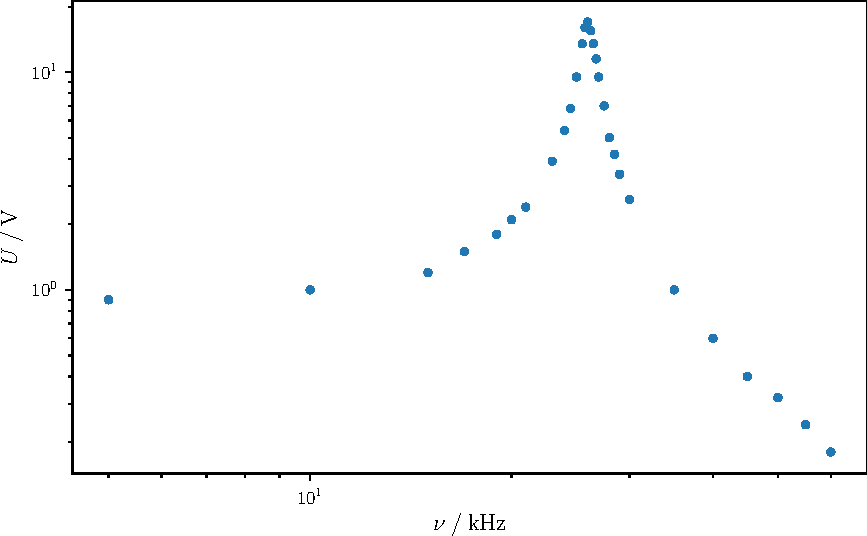
\includegraphics{build/frequence.pdf}
\end{figure}
\begin{figure}
    \centering
    \caption{Bereich um die Resonanfrequenz}
    \label{fig:resonance}
    \includegraphics{build/resonance.pdf}
\end{figure}
\noindent Die Frequenzen $\nu_+ $und $\nu_-$, bei denen die Spannung auf $\sfrac{U_\text{max}}{\sqrt{2}}$ abgefallen ist, liegen bei
\begin{align*}
    \nu_+ &= \SI{26.5}{\kilo\hertz} \\
    \nu_+ &= \SI{25.5}{\kilo\hertz} \; \text{,}
\end{align*}
wodurch sich eine Breite von
\begin{equation*}
    b = \SI{1}{\kilo\hertz}
\end{equation*}
ergibt.
Mit Hilfe der Beziehung \eqref{eqn:güte} lässt sich die Güte zu 
\begin{equation*}
    q = 26
\end{equation*}
errechnen.
Die theoretische Güte, welche sich aus den im Abschnitt \ref{subsec:bauteile} genannten Werten für die Induktivität $L$, 
die Kapazität $C$ und dem Widerstand $R$ errechnen lässt, beträgt 
\begin{equation*}
    q_\text{Theo} = \num{42.41(64)} \; \text{.}
\end{equation*}
Die thereotischen Werte für $\nu_+ $ und $\nu_-$ lassen sich zu 
\begin{align*}
    \nu_{+\text{, Theo}} & = \SI{27.35(4)}{\kilo\hertz}\\
    \nu_{-\text{, Theo}} & = \SI{26.71(4)}{\kilo\hertz} 
\end{align*}
berechnen, was zu einer theoretischen Breite von 
\begin{equation*}
    b_\text{Theo} = \SI{637(4)}{\hertz}
\end{equation*}\\
führt. 
Die Fehler für $q_\text{Theo}$ und $\nu_{\pm\text{, Theo}}$ lassen sich mittels Gaußscher Fehlerfortpflanzung zu
\begin{equation}
    \symup{\Delta} q_\text{Theo} = \frac{1}{\sqrt{RC}} \sqrt{\frac{1}{4LR} \left ( \symup{\Delta} L \right )^2 + \frac{L}{R^3} \left ( \symup{\Delta} R \right )^2 
    + \frac{L}{4C^2R} \left ( \symup{\Delta} C \right )^2} \; \text{,}
\end{equation}
\begin{equation}
    \begin{split}
    \left ( \symup{\Delta} \nu_{+\text{, Theo}} \right )^2= {} & \left ( \symup{\Delta} L \right)^{2} \left(\frac{- \frac{R^{2}}{4 L^{3}} - \frac{1}{2 C L^{2}}}{2 \pi \sqrt{\frac{R^{2}}{4 L^{2}} + \frac{1}{C L}}} - \frac{R}{4 \pi L^{2}}\right)^{2} + \left ( \symup{\Delta} R \right)^{2} \left(\frac{1}{4 \pi L} + \frac{R}{8 \pi L^{2} \sqrt{\frac{R^{2}}{4 L^{2}} + \frac{1}{C L}}}\right)^{2} \\
    & + \frac{\left ( \symup{\Delta} C \right)^{2}}{16 \pi^{2} C^{4} L^{2} \left(\frac{R^{2}}{4L^{2}} + \frac{1}{C L}\right)}
    \end{split} \; \text{,}
\end{equation}
und 
\begin{equation}
    \begin{split}
    \left ( \symup{\Delta} \nu_{-\text{, Theo}} \right )^2= {} & \left ( \symup{\Delta} L \right)^{2} \left(\frac{- \frac{R^{2}}{4 L^{3}} - \frac{1}{2 C L^{2}}}{2 \pi \sqrt{\frac{R^{2}}{4 L^{2}} + \frac{1}{C L}}} + \frac{R}{4 \pi L^{2}}\right)^{2} + \left ( \symup{\Delta} R \right)^{2} \left(- \frac{1}{4 \pi L} + \frac{R}{8 \pi L^{2} \sqrt{\frac{R^{2}}{4 L^{2}} + \frac{1}{C L}}}\right)^{2} \\
    & + \frac{\left ( \symup{\Delta} C \right)^{2}}{16 \pi^{2} C^{4} L^{2} \left(\frac{R^{2}}{4 L^{2}} + \frac{1}{C L}\right)}
    \end{split}
\end{equation}
errechnen.